\hypertarget{sos-s3} {
\subsubsection{Scrum of Scrums}\label{Scrum of Scrums} 
At this point, the team had reorginazed the Epics due to the new architecture 
changes. Having Screen, Bridge and Games as main Epics.
During this sprint, while working on User Story 87, there was a refactoring 
in the architecture due to GUI should be running along with the game. 
Then, in the Lead's Daily a discussion occurred about that change, having it 
as an agreement furthermore, the contract (frontend-library) been terminated in its initial version.
}

\href{https://github.com/Pending-Name-21/arquitecture/pull/12}{Link: GUI Refactor - Pull Request on GitHub}.

\href{https://tree.taiga.io/project/joseluis-teran-coffeetime/taskboard/sprint-3-8974}{Link: User Stories of Sprint 3 on Taiga}.

\hypertarget{burndownchart-s3}{
\subsubsection{Burn Down Chart}\label{Burn Down Chart S3}}
\href{https://tree.taiga.io/project/joseluis-teran-coffeetime/taskboard/sprint-3-8974}{Link: Sprint 3 Board on Taiga}.

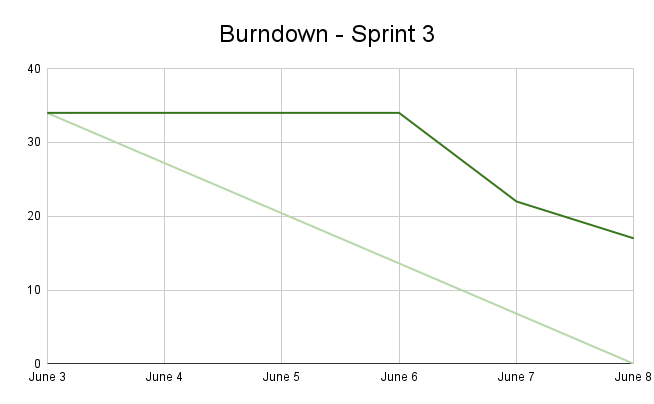
\includegraphics[width=\textwidth]{./artifacts/src/sprint-3/assets/Burndown-Sprint3.png}

\hypertarget{startstopcontinueactionitems-s3}{
\subsubsection{Start-Stop-Continue-Action Items}\label{Start-Stop-Continue-Action Items S3}}
\href{https://miro.com/app/board/uXjVKDO7l8M=/?moveToWidget=3458764590247889881&cot=14}{Link: Start-Stop-Continue-Action Items Sprint 3 on Miro}.

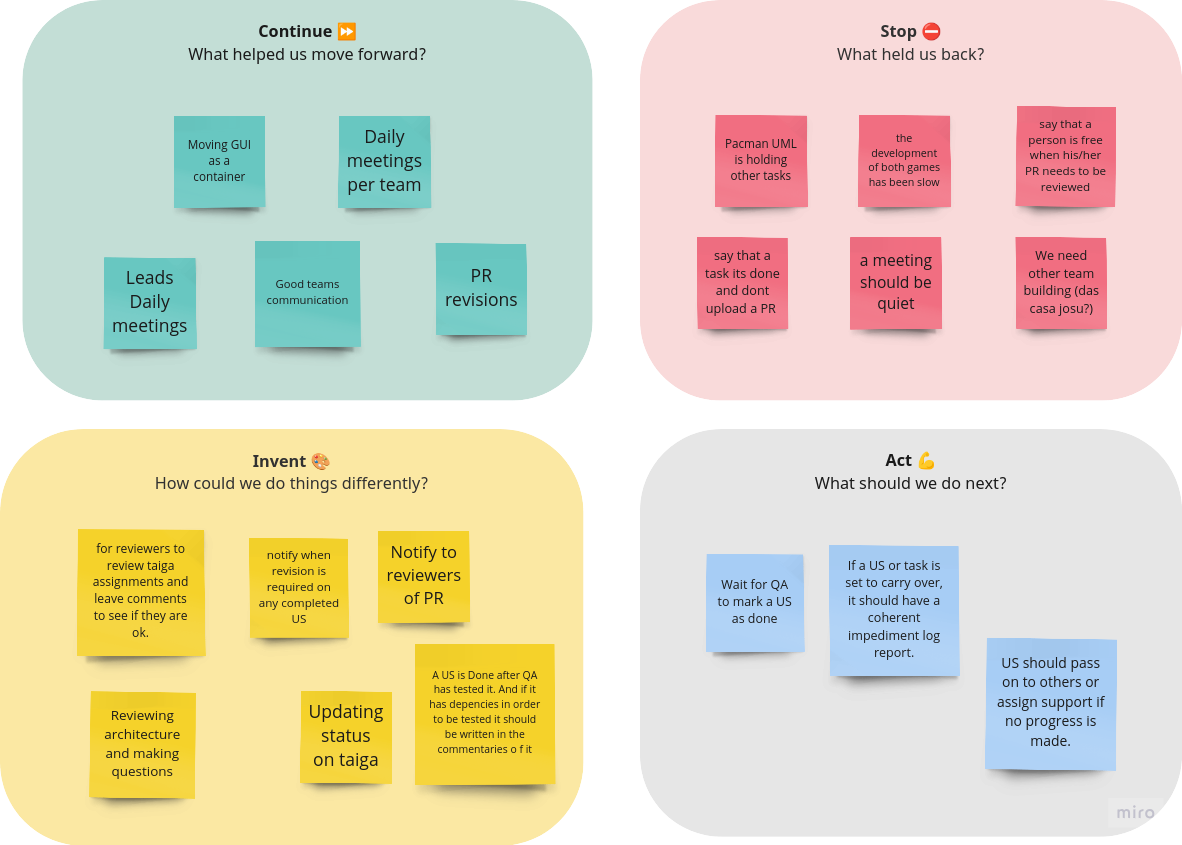
\includegraphics[width=\textwidth]{./artifacts/src/sprint-3/assets/retrospective-s3.png}
